\documentclass[output=paper]{langscibook}
\ChapterDOI{10.5281/zenodo.12090437}
\author{Oksana Laleko\orcid{}\affiliation{State University of New York at New Paltz}}
\title[The complexity of word order change in a flexible system]
      {The complexity of word order change in a flexible system: On stability and variation in heritage Russian word order}
\abstract{The story of heritage languages is often told as a story of grammatical simplification. A substantial body of work has pointed to numerous areas of reduced structural elaboration across heritage language systems, often manifested as a decrease in paradigmatic complexity through the elimination of sub-distinctions in various grammatical categories. Evidence for simplification in the domain of syntagmatic relations, such as in the encoding of information structure relations through word order, is somewhat weaker for heritage languages. This chapter examines the dynamics of heritage language word order change through the lens of Russian. I draw on data from a series of contextualized acceptability judgment tests with homeland Russian speakers and English-dominant heritage Russian speakers at two levels of proficiency, probing the distribution of canonical (SVO) and non-canonical word order structures, including subject-verb inversion (OVS) and object fronting (SOV, OSV). While underrating OVS orders, heritage speakers converge with the controls in their judgments of OSV and SOV sentences, with a trend toward overgeneralization of SOV in high-proficiency speakers. In terms of contextual licensing, focus-driven movement appears more stable than displacement related to givenness. These results offer two important implications. Broadly, they indicate that heritage speakers do not show an across-the-board preference toward SVO syntax, nor do they display a generalized difficulty with information structure marking, suggesting that heritage language word order change should not be viewed narrowly through the lens of simplification, linearization, and pragmatic unmarking. Second, they demonstrate that the facilitation of a non-canonical pattern in a heritage language word order system may occur independently of dominant language transfer effects, bringing into focus other driving forces of language change, including input frequency and universal constituent placement preferences rooted in basic cognitive and communicative principles.}
\IfFileExists{../localcommands.tex}{
  \addbibresource{../localbibliography.bib}
  \usepackage{tabularx,multicol}
\usepackage{url}
\urlstyle{same}
\usepackage{multirow}

\usepackage{stmaryrd}
\usepackage{soul}
\usepackage{enumitem}

\usepackage{siunitx}
\sisetup{group-digits=none}

\usepackage{langsci-optional}
\usepackage{langsci-lgr}
\usepackage{langsci-textipa}
\usepackage{langsci-branding}

\usepackage{tikz-qtree}

\usepackage{pgfplots}
\usepackage{qtree}
\qtreecenterfalse
\usepackage{tree-dvips}
\usepackage{subcaption}

\let\clipbox\undefined
\usepackage{adjustbox}
\usepackage[linguistics, edges]{forest}
\usepackage{langsci-gb4e}

% ORCIDs in langsci-affiliations 
\usepackage{orcidlink}
\SetupAffiliations{orcid placement=before}
\definecolor{orcidlogocol}{cmyk}{0,0,0,1}
\RenewDocumentCommand{\LinkToORCIDinAffiliations}{ +m }
  {%
    \orcidlink{#1}\,%
  }

  \newcommand*{\orcid}[1]{}


\makeatletter
\let\thetitle\@title
\let\theauthor\@author
\makeatother

\newcommand{\togglepaper}[1][0]{
   \bibliography{../localbibliography}
   \papernote{\scriptsize\normalfont
     \theauthor.
     \titleTemp.
     To appear in:
     E. Di Tor \& Herr Rausgeberin (ed.).
     Booktitle in localcommands.tex.
     Berlin: Language Science Press. [preliminary page numbering]
   }
   \pagenumbering{roman}
   \setcounter{chapter}{#1}
   \addtocounter{chapter}{-1}
}

\newbool{bookcompile}
\booltrue{bookcompile}
\newcommand{\bookorchapter}[2]{\ifbool{bookcompile}{#1}{#2}}


\forestset{
  my nice empty nodes/.style={% modified from manual page 52
    for tree={
      calign=fixed edge angles,
      calign angle=50,
    },
    delay={
      where n children=0{
        if content={}{
          content=\strut,
          anchor=north,
        }{
          align=center
        },
      }{
        if content={}{
          shape=coordinate,
          for parent={
            for children={
              anchor=north
            }
          }
        }{}
      }
    },
  },
  my pretty nice empty nodes/.style={
    for tree={
      calign=fixed edge angles,
      calign angle=50,
      parent anchor=south,
      delay={
        where n children=0{
          if content={}{
            content=\strut,
            anchor=north,
          }{
            align=center
          },
        }{
          if content={}{
            inner sep=0pt,
            edge path={\noexpand\path [\forestoption{edge}] (!u.parent anchor) -- (.south)\forestoption{edge label};}
          }{}
        }
      }
    }
  }
}


\newcommand{\sem}[1]{\mbox{$[\![$#1$]\!]$}}
\newcommand{\type}[1]{\ensuremath{\left \langle #1 \right \rangle }}
\newcommand{\lam}{\ensuremath{\lambda}}
\renewcommand{\and}{$\wedge$ }
\newcommand{\bex}{\begin{exe}}
\newcommand{\eex}{\end{exe}}
\newcommand{\bit}{\begin{itemize}}
\newcommand{\eit}{\end{itemize}}
\newcommand{\ben}{\begin{enumerate}}
\newcommand{\een}{\end{enumerate}}

\newcommand{\gcs}[1]{\textcolor{blue}{[gcs: #1]}}
\newcommand{\ash}[1]{\textcolor{orange}{[ash: #1]}}
\newcommand{\ngn}[1]{\textcolor{purple}{[ngn: #1]}}

\newcommand{\firstrefdash}{}


\forestset{
fairly nice empty nodes/.style={
delay={where content={}
{shape=coordinate, for siblings={anchor=north}}{}},
for tree={s sep=4mm}
}
}


 
  \input{../localhyphenation} 
  \togglepaper[1]%%chapternumber
}{}

\begin{document}
\renewcommand{\lsChapterFooterSize}{\footnotesize}
\maketitle


\section{Introduction}\label{sec:laleko:1}

Within the burgeoning literature on heritage languages and their linguistic properties, two overarching and partially intertwined themes have recently come to dominate the scholarly landscape. On the one hand, many researchers have pondered whether or not the presently available empirical data on structural properties of heritage languages allow for broader generalizations bearing on the issue of heritage language typology. Is it in principle possible to identify features, processes, and patterns that would prove characteristic of heritage languages as a linguistic phenomenon, and if so, what is the nature of these properties and how would they vary along a continuum of heritage grammars, including its diachronic (i.e., acquisition and transmission) and synchronic (i.e., proficiency and individual variability) dimensions? While a number of researchers have suggested that such generalizations are conceivable -- at the very least, for certain domains of heritage language design (\citealt{BenmamounPolinsky2013, LohndalWestergaard2019, PolinskyScontras2020}), it is clear that much cross-linguistic work remains to be done on the empirical front in order to bring the existing proposals up to the highest levels of explanatory robustness through rigorous testing under typologically and sociolinguistically varied conditions.

The second theme, and one that the present paper takes as its primary impetus, concerns the long-standing conceptualization of heritage language change as a unidirectional process of a decrease in linguistic complexity. Building on traditions rooted in decades of work on language obsolescence and attrition studies (\citealt{Dorian1989, Sasse2001}), theoretical models of heritage language competence have drawn heavily on linguistic research that has attended most extensively to areas of reduced structural elaboration across heritage language systems. Setting aside for a moment issues related to heritage language processing, existing representational models have, accordingly, tended to construe heritage language grammars as smaller, more economically organized networks of structures with (i)~an overall lower degree of paradigmatic complexity due to the elimination of sub-distinctions in grammatical categories (e.g., case, gender, aspect), and (ii)~tighter and more locally defined syntagmatic relationships. As discussed recently in \citeauthor{LalekoScontras2021} (\citeyear{LalekoScontras2021}; see also other papers in the special issue of the \textit{Heritage Language Journal} on heritage language complexity), few studies have systematically accounted for instances of complexity invariance, indicative of areas of stability in heritage language transmission, and even fewer have turned their attention to processes of complexification arising in heritage language systems. Yet, there is no a priori reason to expect complexity-preserving and even complexity-increasing mechanisms of change to be inoperative in heritage language contexts. Since the blossoming of historical linguistic studies in the nineteenth century, the prevalence of these processes in language evolution has been well recognized (e.g., \citealt{Lightfoot1991}), including their manifestations in situations of contact-induced change, of which heritage languages are a particular, and in fact very prominent, case.

Building on insights from typological and historical linguistic studies, one may turn attention to a number of language-internal and external factors to identify possible triggers of complexity-producing change in heritage languages. Elements of complexification could arise, for instance, as by-products of compensatory trade-offs across various linguistic sub-domains affected by selective loss of forms and subsequent redistribution of functions correlated with the retained forms. In the same vein, form-preserving and strengthening effects could stem from cross-linguistic influence on the heritage language of other languages spoken in the same linguistic niche, including most notably the societally dominant language and, a less-often explored possibility, other minority languages competing for the speakers’ cognitive resources. Likewise, one could look for signs of complexification in the form of original innovations reflecting the unique socio-demographic and linguistic conditions in which heritage grammars are constructed, a line of inquiry that seems particularly promising for heritage languages developing within stable diasporic speech communities and transmitted intergenerationally. Whatever the extent and primary source(s) of complexification phenomena turn out to be in heritage languages, these general considerations warrant a more nuanced approach to modeling heritage language change, one in which the predicted structural outcomes would rest on a more explicit recognition of the multi-dimensional and multi-directional nature of language change as a linguistic process.

Taking as a point of departure the prevailing assumption that the story of heritage languages is largely a story of grammatical simplification, this chapter aims to expand the conception of heritage language change as a phenomenon of much broader scope. As one step towards this goal, I examine the dynamics of word order change in heritage Russian, drawing on data taken to represent two distinct stages of change from a cross-sectional standpoint, compared to the homeland baseline. As I detail further below, word order variation in Russian, along with other Slavic languages, provides a fitting opportunity for investigations of heritage language word order change through the lens of complexity change: As discourse-configurational systems with an underlying SVO typology, Slavic languages make heavy use of scrambling (\citealt{Ross1967}) to encode information structure relations in discourse, yielding virtually every possible configuration of clausal constituents possible and communicatively desirable under the right discourse-pragmatic conditions. Given that most theoretical studies converge on the assumption that non-canonical (i.e., scrambled) sentences are more complex in Russian than those following the canonical order (\citealt{Sekerina2003}: 302), the study of variation in this domain of a heritage language system emerges as a \textit{bona fide} case of complexity variation.

In order to position the above claim more directly within the existing models of linguistic complexity, we may wish to draw a further distinction between \textit{absolute} and \textit{relative} complexity, two conceptualizations of complexity that have been utilized, independently of each other or jointly, across a number of linguistic fields in an attempt to establish specific, practically useful metrics serving to demarcate what one would consider more or less complex in language structure and/or language use (see \citealt{LalekoScontras2021} for a recent discussion). Within this dichotomy, the former notion of absolute complexity has been operationalized most prominently in typological and diachronic studies focused on the structural characteristics of linguistic systems and subsystems, while the latter notion of relative complexity has gained much ground in psycholinguistic work and research on language acquisition, taking the standpoint of the language user as the key benchmark in assessing linguistic complexity.

Drawing on metrics advanced within each of these frameworks, and assuming SVO as the underlying basic order, one would only need to take a very broad glance at the existing theoretical analyses of scrambling in Slavic to observe that the derived status of discourse-dependent orders places them onto the higher end of the complexity scale relative to the canonical, base-generated order. In the absolute, system-centered sense, the increased complexity associated with discourse configurationality is suggested by a range of factors including, but not limited to: the added structural complexity of the projections hosting the scrambled components, the additional movement operations involved in their relocation, the overall greater number of rules that must be specified to license the occurrence of scrambled orders, the less transparent (i.e., less faithful) relationship between the underlying and surface representations, or, from a cross-linguistic perspective, their higher typological markedness.\footnote{The last observation does not hold for SOV orders (\citealt{Greenberg1963, Dryer2013Order}).} From the relative, or user-based, perspective, adopted in many processing-based models of scrambling, non-canonical sentences come out as more complex as well: time and again, structures with displaced constituents have been shown to engage more computational and working memory resources than those following canonical orders (\citealt{Gibson1998, Just1996}).

In light of these considerations, and under the conception of heritage language change as a shedding of complex structures, word order change in a flexible system should look like a process of word order levelling, manifested in the weakening and loss of non-canonical orders in favor of the default (here: least contextually-bound) pattern. In situations of a shared default between the contact languages, which is the case for the Russian-English dyad examined here, it is the predominant SVO order that emerges as a prime candidate for replacing the scrambled orders in the simplified system, predicting exponentially degraded ratings of non-SVO orders in both heritage speaker groups. Conversely, if heritage language word order change involves complexity-preserving mechanisms as part of its process, the affected grammars may retain or even make greater use of structures falling under the umbrella of non-canonical orders, resulting in a distinct – but not necessarily universally simpler – system. To anticipate the presentation of the results that follows, it is the latter scenario that is borne out empirically.

The rest of the chapter is structured as follows. \sectref{sec:laleko:2} brings into focus the relevant theoretical generalizations and empirical findings pertaining to word order variation in Russian. In \sectref{sec:laleko:3}, I offer a concise review of representative existing studies on word order change in heritage languages, highlighting findings that bear most closely on the phenomena addressed in this study. \sectref{sec:laleko:4} presents the methodology and results of the study, while \sectref{sec:laleko:5} discusses its findings and their implications.

\section{Theoretical and experimental approaches to word order variation in Russian}\label{sec:laleko:2}

At least since the writings of the Prague School linguists (\citealt{Mathesius1947, Firbas1964}), it has been recognized that the surface linearization of clausal constituents (and their parts) in Slavic languages, including Russian, is strongly regulated by the communicative principles related to the encoding of information structure. However, the exact nature of the encoded categories and the mechanism(s) of their impact on the linguistic structure remain subject to lively debates to this date. Broadly, analyses of word order variation in Russian may be conceived of as occupying a niche along the spectrum between two poles: functionalist approaches, striving to identify the elements of discourse and pragmatic structure correlated with word order variation, and syntactic approaches, focused on working out the linguistic principles involved in deriving the resulting structures. The brief exposition of the literature in this section highlights the key insights gained from both perspectives.

Among the functionalist accounts, one of the central questions has been the problem of conceptualizing the relevant information-structural relations responsible for the flexibility of surface orders in Slavic. While converging on the observation that sentences in languages like Russian tend to be organized so as to allow for a predictable ordering between parts that are relatively less informative and parts that are relatively more informative, with the former preceding the latter, a number of dichotomies have been proposed to capture these relations. Pairs of terms such as \textit{theme} and \textit{rheme}, \textit{topic} and \textit{comment}, \textit{givenness} and \textit{newness}, \textit{background} and \textit{focus}, \textit{presupposition} and \textit{focus}, \textit{topic} and \textit{focus} have all been used for this purpose, sometimes interchangeably but often with important differences in theoretical assumptions (see \citealt{GundelFretheim2004} for a terminological overview). In keeping with the general rule of linearly increasing informativeness as the primary guiding principle of sentence structuring in Russian (\citealt{Gundel1988}), several scholars have further expanded the traditional binary partition into a tripartite template, in which the discourse-neutral information may be hosted medially between the two informationally-distinguished parts as illustrated in \REF{ex:laleko:1} below (\citealt{Brun2001, King1995}):

\ea%1
    \label{ex:laleko:1}
           (Topic) – (discourse-neutral information) – focus
\z


\begin{sloppypar}
In accordance with this structuring, constituents occurring at the right edge of the clause in Slavic are most straightforwardly interpreted as carrying new information, while constituents in earlier positions are more easily assigned a discourse-neural or given status. To facilitate such interpretation, constituents base-generated elsewhere in the clause – but associated with new information (i.e., presentational) \textit{focus} – may surface at the right edge; conversely, constituents that are \textit{given} (e.g., by virtue of having been mentioned in prior discourse or otherwise accessible) can shift away from their canonical right-edge positions, leaving other material in the focus domain. These scenarios are illustrated in the examples (\ref{ex:laleko:2}--\ref{ex:laleko:4}) below. In \REF{ex:laleko:2}, the SVO sentence is presented in a broad-focus (i.e., “out of the blue”) context, such that all of its constituents represent new information. In \REF{ex:laleko:3} and \REF{ex:laleko:4}, presentational focus rests narrowly on the subject or the verb, respectively; all remaining constituents in the answer sentences are discourse-given by virtue of appearing in prior context. It should be noted that the movement involved in the non-canonical examples below is not of obligatory nature, making SVO orders possible across all contexts, with the focused constituent receiving prosodic stress \textit{in situ} (see, e.g., \citealt{Jasinskaja2016}).
\end{sloppypar}

\ea%2
    \label{ex:laleko:2}
\ea
\gll   Kakie   novosti?\\
what  news-\textsc{fem}.\textsc{pl}\\
\glt ‘What’s new?’

\ex
\gll Papa    prodal      mašinu.\\
    dad-\textsc{nom.sg}  sell-\textsc{past.sg}    car-\textsc{acc}.\textsc{sg}\\\jambox*{SVO}
\glt     ‘Dad sold the car.’
    \z
\z

\ea%3
    \label{ex:laleko:3}
\ea
\gll   Kto     prodal      mašinu?      \\
who-\textsc{nom}  sell-\textsc{past.sg}    car-\textsc{acc}.\textsc{sg}\\
\glt ‘Who sold the car?’

\ex
\gll Mašinu  prodal      papa.\\
  car-\textsc{acc}.\textsc{sg}  sell-\textsc{past.sg}    dad-\textsc{nom.sg}\\\jambox*{OVS}
\glt   ‘Dad sold the car.’
\z
\z

\ea%4
    \label{ex:laleko:4}
\ea
\gll    Čto   papa    sdelal    s  mašinoj?\\
    what  dad-\textsc{nom.sg}  do-\textsc{past.sg}  with  car-\textsc{acc.sg}  \\
\glt    ‘What did dad do with the car?’

\ex
\gll  Papa    mašinu    prodal.\\
    dad-\textsc{nom.sg}  car.\textsc{acc}.\textsc{sg}  sell-\textsc{past.sg}\\\jambox*{SOV}
\glt     ‘Dad sold the car.’

\ex
\gll Mašinu  papa    prodal.\\
  car-\textsc{acc.sg}  dad-\textsc{nom.sg}  sell-\textsc{past.sg}\\\jambox*{OSV}
\glt    ‘Dad sold the car.’
\z
\z

Within the syntactically-oriented strand of research on dis\-course-con\-fig\-u\-ra\-tion\-al\-i\-ty in Slavic, we once again find a spectrum of proposed models that vary in their assumptions and conclusions, ranging from those that bring the discourse requirements on scrambling directly into the syntax (\citealt{King1995}) to those postulating a separate abstract level of representation, such as Functional Form (\citealt{Bailyn1995}), Information-Structure (\citealt{JunghannsZybatow1997}), or I-Structure (\citealt{Kondrashova1996}), at which word order is linearized in accordance with the information-structural partition of the utterance. The nature and directionality of operations leading to such linearization are even less fully understood. Consensus has not been reached on such fundamental issues as whether the categories of topic and focus occupy dedicated syntactic projections (\citealt{King1995, Dyakonova2009}), are associated with features not linked to particular projections (\citealt{Kondrashova1996}), or are split such that only topics, but not foci, project syntactically (\citealt{JunghannsZybatow1997}); whether all movements are leftward (\citealt{Slioussar2007}) or are bi-directional (\citealt{Sekerina1997}); and how the relevant operations are to be motivated (e.g., \citealt{Titov2020}).

Despite these many points of disagreement, most existing analyses converge globally on the observation that while the surface ordering of constituents in Russian marks their information-structural roles, the underlying configuration of the Russian clause reflects the grammatical functions of the arguments, with SVO as the underlying, basic pattern (however, see \citealt{King1995} for arguments in favor of treating Russian as a VSO language in which subjects move out to serve as topics). This theoretical consensus is supported by experimental observations. Looking at the parsing strategies employed by Russian speakers in processing basic and scrambled constructions, \citegen{Sekerina1997} eye-tracking study provided psycholinguistic evidence for SVO serving as the basic, discourse-neutral variant within the Russian word order system. Prior offline linguistic studies with monolingual Russian-speaking children and adults have reached the same conclusion. For example, in a repetition task reported in \citet{Bailyn1995}, Russian-speaking children between ages 3.8 and 5.5 demonstrated higher accuracy rates for SVO orders (83\% correct) compared to non-SVO orders (40\% correct). Studies with adults have similarly pointed to the predominance and functional versatility of the SVO pattern in Russian. \citet{HoldenKrupp1987}, for instance, conducted a written acceptability study in which participants were asked to rank the six possible orders appearing in neutral and discourse-specific contexts, assuming that all sentences are to be read with neutral intonation. Across all contexts, SVO emerged as the preferred pattern for Russian monolingual adults. In a more recent study with adult monolinguals, \citet{Kallestinova2007} similarly found 98.9\% of context-neutral transitive sentences to be produced in SVO form. Across various discourse contexts, the Russian speakers were overall found to favor SVO, OVS, and SOV orders in production, and while the remaining orders (VSO, VOS, and OSV) were not produced consistently, they were still recognized as acceptable on grammaticality judgment tasks (\citealt{Kallestinova2007}).

Investigations of corpus data have generally been in line with the experimental findings discussed above; however, they have also unveiled substantial variation in the frequency of non-canonical orders in written and spoken Russian. According to a synopsis of prior corpus studies presented in \citet[260]{MillerWeinert1998}, both modalities generally favor SVO as the predominant order, but with a quantitatively significant decrease in its occurrence in the spoken language: for (mostly) written Russian, SVO (79\%), OVS (11\%), OSV (4\%), VOS (2\%), SOV (1\%), and VSO (1\%); for spoken Russian, SVO (42\%), SOV (34\%), OSV (11\%), and OVS (3\%). A quick comparison of the distributional patterns for the remaining orders reveals a bias toward written registers for OVS structures and an association with spoken language for object-fronted orders (SOV, OSV). In a more recent analysis of the Russian National Corpus, \citet{Billings2015} reports the following word order frequencies based on a sample of 500 transitive sentences: SVO (89.6\%), SOV (4.4\%), OVS (2.4\%), OSV (1.8\%), VSO (1.6\%), VOS (0.2\%). While suggesting an overall more rigid sentence structure than one reported in prior studies, this pattern aligns well with the production results of \citegen{Kallestinova2007} study, which identified the same three top orders for Russian. Since the majority of sentences in \citegen{Billings2015} sample (74.4\%) represent non-academic texts, the distribution of these orders by register, while suggestive of register-based variation, is presented in tentative terms. However, within the data for non-academic texts, comprising the majority of the sample, SVO, SOV, OVS, and OSV configurations emerge as the most productive orders (\citealt{Billings2015}: 36). It is these four orders in Russian that are investigated in the present study.

\section{Word order in heritage languages: A snapshot of current research}\label{sec:laleko:3}

Whether or not heritage languages preserve the word order(s) generated in their corresponding baselines is a question that has received increasing attention from researchers in recent years, partly due to a spike in interest in the status of interface properties in bilinguals, triggered by several influential proposals, and partly as a result of a steadily improving access to heritage language corpora that has made such explorations possible (see \citealt{Kisselev2021}). A substantial number of word order studies have turned the spotlight on syntactically-driven phenomena (e.g., \citealt{HoppPutnam2015, KühlPetersen2018, WestergaardLohndal2019} on V2, \citealt{AnderssenWestergaard2020} on the interactions of pronominal argument placement with negation), finding these properties to be somewhat vulnerable but overall not drastically affected in the heritage varieties under investigation. In what follows, however, I will limit my literature survey to studies that have delved explicitly into the effects of information structure on word order variation in heritage language production and comprehension.

Within this cohort of studies, the encoding of the two key dimensions of information structure, focus and topicality (or givenness), have tended to be considered independently of each other, with the majority of published work focusing on the principles governing the encoding of the most informationally salient linguistic elements across heritage language systems. Such “focus on focus” bias has left significant gaps in our understanding of heritage language strategies related to the syntactic expression of givenness. Despite the asymmetry in the available body of work, the overall results in both domains of inquiry have not reached a consistent level of uniformity across language dyads, proficiency levels, linguistic contexts examined, and experimental techniques employed for data collection, highlighting the need for a more synergistic evaluation of these factors in future studies.

With respect to the marking of focus, for example, even within a single narrowly defined domain, such as the distribution of SV and VS orders with intransitive verbs in relation to the informational prominence of the subject, one finds a considerable \textit{concordia} \textit{discors} across the scholarly terrain. Working with English-dominant heritage speakers, \citet{ZapataToribio2005} and \citet{Laleko2022} detected no consistent influence of focus, even in advanced speakers, on subject position with unergative predicates (which do not independently trigger VS) in heritage Spanish and Russian, respectively. However, \citet{PradaPérezCabo2012} reported target-like contrasts in the same domain in English-dominant Spanish heritage speakers at three levels of proficiency, and \citet{vanOschSleeman2018Subject} documented an increase in the acceptability of the non-canonical VS orders in Dutch-dominant heritage Spanish speakers, an effect the authors attribute to dominant language influence. Expanding the scope of inquiry to transitive and di-transitive structures, studies by \citet{Hoot2017} and  \citet{GómezSolerCabo2018} on Spanish in the U.S. reported strong effects of focus on subject and object placement in heritage speakers, a finding paralleled in \citet{IoninStyrina2021} for U.S. Russian. At the same time, using processing measures, \citet{SagarraSanchezBel2019} detected lower accuracy rates for OVS structures in a self-paced reading study of U.S. Spanish. Similarly, \citet{Hoot2019} demonstrated target-like felicity judgments for constructions involving focus-movement in English-dominant heritage speakers of Hungarian, but the interpretations of these structures were found to differ from those in baseline speakers.

Little work has been done comparing the use of canonical and non-canonical orders across speakers of the same heritage language with different contact languages, but such studies can be pivotal in charting out the role of cross-linguistic influence on the development of the relevant constructions in the heritage language. \citet{ZubanEtAl2021} examined the production of SVO and OVS orders in heritage Russian in Germany and the U.S. and found a difference between German-dominant and English-dominant speakers, with a reduction in the use of OVS orders in the latter group. Earlier production studies of heritage Russian in the U.S. documented a similar quantitative decrease in the use of OVS and other non-canonical constructions in the oral narratives produced by heritage speakers (\citealt{IsurinIvanovaSullivan2008, Ivanova-Sullivan2014, LalekoDubinina2018, Polinsky2008Heritage}) – a pattern also shown to hold in written essays produced by heritage Russian learners (\citealt{Kisselev2019}). Yet, in contrast to these college-age English-dominant heritage writers of Russian, their slightly younger German-dominant peers were found to maintain and even amplify the high flexibility of word order in Russian, with some evidence of a carry-over of the propensity for V-final orders to both main and subordinate clauses (\citealt{BrehmerUsanova2015}).

The effects of topicality or givenness on the placement of constituents have not been examined as extensively for heritage languages; still, a similarly non-uniform picture emerges from the examination of the presently available data, limited to date mostly to the study of topicalization and clitic dislocation phenomena in Spanish. Based on reduced occurrence and diverging judgements of topicalization and clitic left dislocation in heritage Spanish speakers, \citet{ZapataToribio2005} argue for permeability of interface domains to cross-linguistic influence in bilinguals. Investigations of clitic left dislocations in \citet{Montrul2010Dominant, Montrul2010How} further point to significant proficiency effects in the acquisition of these structures in the heritage language. Conversely, looking at clitic right dislocation, a rare construction employed for topicalization,  \citet{LealSlabakova2014} report no proficiency effects on the ratings of heritage Spanish speakers, who demonstrated target-like felicity contrasts in their judgments at intermediate and advanced levels of proficiency. More recently,  \citet{LealMéndezSlabakova2015} and \citet{Sequeros-ValleCabrelli2020} provide further experimental evidence of convergence between heritage and baseline Spanish speakers on topic constructions by examining clitic-doubled left dislocations, which bear an anaphoric relation to the discourse context. While overextending these structures to non-anaphoric contexts in acceptability judgments, heritage speakers are overall found to perform on par with baseline speakers in making context-appropriate distinctions in their use, with differences between groups attributed to task effects rather than to gaps in the underlying knowledge of the construction in heritage bilinguals.

In summary, despite growing attention of researchers to the issue of information structure marking through word order in heritage languages, the overall picture remains rather mixed, with much work remaining to be done to reach a more balanced assessment of the relevant phenomena across languages, for speakers at various proficiency levels, and via methodologically diverse techniques. As the brief synopsis above suggests, for Russian in particular, very little work has extended beyond oral or written production to examine constraints on the occurrence of basic and discourse-dependent orders in heritage speakers, and no studies have experimentally investigated parallels between the syntactic encoding of focus and givenness in speakers at distinct proficiency levels. This study seeks to accomplish this goal.

\section{The study}\label{sec:laleko:4}

The experimental data presented in this section come from a larger research project designed to investigate syntactic and prosodic realization of information structure in Russian as a heritage and second language. Here, I draw on three written contextualized acceptability judgment experiments to examine the effects of focus and givenness on constituent placement preferences in homeland and heritage language speakers. The role of focus is addressed in the first experiment, comparing ratings for SVO and OVS orders in two different information-structural configurations: under broad focus, as illustrated in example \REF{ex:laleko:2} above, and under narrow presentational focus on the subject, as shown in \REF{ex:laleko:3}. The effects of givenness are the main focus of the second and third experiments, aimed to test the speakers’ object placement preferences and targeting SOV and OSV constructions, respectively. Building on prior findings attesting to a correlation between VO/OV orders and object givenness in Russian (\citealt{Sirotinina1965, Slioussar2007}), ratings for sentences with postverbal and preverbal accusative objects are obtained in two conditions: under broad focus, where the entire sentence, including the object constituent, carries new information, and under narrow focus on the verb, in which the object constituent represents given (i.e., old, known, shared, previously mentioned, accessible from prior discourse) information, as demonstrated in \REF{ex:laleko:4} above. Taking into account the frequently observed tendency for the preverbal Russian objects to be pronominalized (\citealt{MillerWeinert1998}: 260), the object-given condition in the second and third experiments comprised two sub-conditions, with nominal and pronominal objects analyzed separately from each other.

Considering the scarcity of controlled experimental data on word order preferences in heritage Russian, the main research questions of the study were formulated broadly: (i) overall, how do heritage speakers of Russian compare to homeland speakers in their syntactic encoding of focus and givenness; (ii) what effect does heritage language proficiency play in both domains? However, keeping in mind the issues addressed in this chapter, each of these broad questions has been operationalized into predictions that directly engage the problem of complexity in heritage language change. First, if word order restructuring proceeds in the direction of simplification, manifested as the amplification of the syntactic default shared by the bilinguals’ word order grammars, we should observe a reduction in the acceptance of scrambled orders in the data from heritage speakers in comparison to the baseline. Second, taking as a starting point the traditional conception of heritage language proficiency as a linear continuum that displays greatest signs of restructuring at its lowest level and incrementally converges with the baseline at its highest level (cf. the creole continuum model in \citealt{Bickerton1975} and its reconceptualization for heritage languages in \citealt{PolinskyKagan2007}), the word order system instantiated in the grammars of the higher-proficiency speakers should be closer to the baseline system than one constructed by speakers at a lower point on the continuum.

To test these predictions, acceptability ratings were gathered from forty-two adult speakers of Russian, including twenty-seven English-dominant heritage speakers (mean age = 19.4) and fifteen monolingually raised Russian-speaking controls (mean age = 24). All heritage speakers identified English as their primary and most frequently used language of daily communication and designated Russian as their non-dominant and less frequently used language (mean of average daily use = 23.7\%). Consistent with the canonical profile of early imbalanced naturalistic bilinguals (\citealt{AalberseMuysken2019, Montrul2016, Polinsky2018}), all heritage speakers in the study reported hearing and speaking Russian in early childhood, followed by an increase in the use of English coinciding, on average, with the age of entering the public school system (mean age of switch to English = 4.5). In contrast, all speakers in the control group reported Russian as the only language used in all daily communication and provided at-ceiling proficiency self-ratings across the four key areas of linguistic competence (understanding, speaking, reading, and writing Russian). The heritage speakers’ self-assessments of the same four areas revealed the expected imbalance between skills acquired in a naturalistic environment (mean rating = 8.2 on a 10-point scale for understanding, mean rating = 7.1 for speaking) and those associated with explicit, formalized learning (mean rating = 6.5 for reading, mean rating = 6 for writing), suggesting a direct correlation between the speakers’ degree of confidence in their linguistic abilities and the extent of their exposure to contexts in which these abilities are typically acquired.

In addition to the self-ratings of the Russian language proficiency obtained as part of the socio-demographic questionnaire, all participants completed an independent proficiency test designed to assess the speakers’ morpho-syntactic knowledge across several grammatical domains previously shown to undergo restructuring and correlate with proficiency in heritage language speakers (\citealt{Polinsky2018}). The test consisted of ten sentences containing violations in the areas of grammatical gender, subject-verb agreement, and pro-drop. On the basis of the obtained proficiency scores (for monolinguals, the mean score was predictably low at 1.6 on a 1--5 Likert scale), the heritage speakers were divided into two groups, yielding a higher-proficiency group of 12 speakers (mean score of 1.8) and a lower-proficiency group of 15 speakers (mean score of 2.8), with a statistically significant difference obtained between the two heritage speaker groups based on proficiency ($t(22)=-7.2$, $p<0.01$). Participants with a mean proficiency score of 4.0 or above were not included in the study.

The speakers rated 48 target sentences, intermixed with 60 fillers and presented in a randomized manner in Experigen (\citealt{BeckerLevine2013}). The stimuli were presented to the participants as question-answer sequences, with one question followed by two answer choices with a 5-point Likert scale appearing next to each of the two answers. This design was deemed optimal to ensure that any differences in the participants’ ratings of the relevant word order configurations reflected their judgments of word order proper, keeping the lexical and morphological information identical between the canonical and non-canonical sentences being evaluated.

The means for the relevant conditions of the study, presented in Figures~\ref{fig:laleko:1}--\ref{fig:laleko:3} below, were analyzed statistically using Welch’s unequal variances $t$-tests. First, I present the results on the syntactic encoding of focus in the three varieties\footnote{In all figures, the data are presented in the following order: N = homeland speakers, HL(h) = higher-proficiency heritage speakers, HL(l) = lower-proficiency heritage speakers.} of Russian under investigation, comparing SVO and OVS sentences under broad focus and under narrow focus on the subject constituent (\figref{fig:laleko:1}).

\begin{figure}
\caption{\label{fig:laleko:1}Ratings for SVO and OVS sentences in all-new-information and subject-focus contexts}
  \footnotesize
  \begin{subfigure}[b]{.4\textwidth}
  \centering
  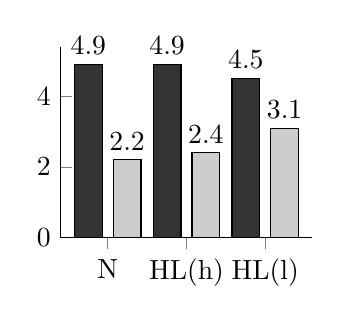
\begin{tikzpicture}
  \selectcolormodel{gray}
    \begin{axis}[ybar=4pt,
            x=1cm,
            ymin=0,
            symbolic x coords = {N,{HL(h)},{HL(l)}},
            xtick=data,
            axis lines*=left,
            nodes near coords,
            height=4cm,
            width=5cm,
            enlarge x limits=0.3
        ]
    \addplot[fill=black!80, draw=black] coordinates {
        (N,4.9)
        ({HL(h)},4.9)
        ({HL(l)},4.5)
    };
    
    \addplot[fill=black!20, draw=black] coordinates {
        (N,2.2)
        ({HL(h)},2.4)
        ({HL(l)},3.1)
    };
    \end{axis}
  \end{tikzpicture}
  \caption{Broad}
  \end{subfigure}%
  \begin{subfigure}[b]{.6\textwidth}
  \centering
  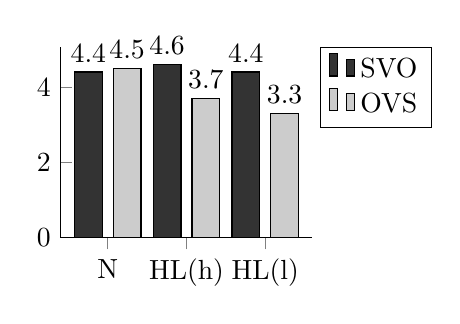
\begin{tikzpicture}
    \begin{axis}[ybar=4pt,
            x=1cm,
            ymin=0,
            symbolic x coords = {N,{HL(h)},{HL(l)}},
            xtick=data,
            axis lines*=left,
            nodes near coords,
            height=4cm,
            width=5cm,
            enlarge x limits=0.3,
            legend pos = outer north east
        ]
    \addplot[fill=black!80, draw=black] coordinates {
        (N,4.4)
        ({HL(h)},4.6)
        ({HL(l)},4.4)
    };
    \addlegendentry{SVO}

    
    \addplot[fill=black!20, draw=black] coordinates {
        (N,4.5)
        ({HL(h)},3.7)
        ({HL(l)},3.3)
    };
    \addlegendentry{OVS}
    \end{axis}
  \end{tikzpicture}
  \caption{Narrow}
  \end{subfigure}
%%\includegraphics[width=\textwidth]{figures/LalekoThecomplexityofwordorderchangeinaheritagelanguagesettingfinal-img001.svm}
\end{figure}


In line with the theoretical generalizations about the unmarked, contextually unrestricted status of SVO in Russian, all participants demonstrated very high acceptance rates for SVO orders across all experimental conditions. Furthermore, both the homeland speakers and the higher-proficiency heritage speakers displayed nuanced judgments of OVS orders based on information structure, rating these structures significantly higher under narrow focus than under broad focus: controls ($t(82.2)=-10.3$, $p<0.01$); HL(h) ($t(51.8)=-3.7$, $p<0.01$). These results indicate that the interaction of OVS orders and subject focus, frequently discussed in the theoretical literature on Slavic and confirmed experimentally in this study, is actively operative at high levels of heritage language proficiency. In contrast, the lower-proficiency heritage speakers rated OVS orders similarly in broad-focus and narrow-focus conditions: ($t(61.2)=-0.4$, $p>0.05$), suggesting no sensitivity to this information-structural constraint in these speakers’ grammars. While attesting to baseline-like principles on the occurrence of OVS orders in high-proficiency speakers, the results nevertheless reveal a quantitative reduction in the acceptability of these orders by heritage speakers at both levels of proficiency, compared to the homeland speakers. Thus, in the narrow focus condition: controls vs. HL(h) ($t(63.08)=3.01$, $p<0.01$); controls vs. HL(l) ($t(76.8)=4.46$, $p<0.01$). 

The remaining data bear on the encoding of givenness in the varieties of Russian examined. First, I outline the results obtained for SVO and SOV sentences presented in all-new-information contexts and in contexts that identify the object constituent as discourse-given. In the latter condition, data for sentences with nominal and pronominal objects are presented separately (\figref{fig:laleko:2}).

\begin{figure}
\footnotesize
\caption{\label{fig:laleko:2}Ratings for SVO and SOV sentences in all-new-information and object-given contexts}
 \begin{subfigure}[b]{.3\textwidth}
  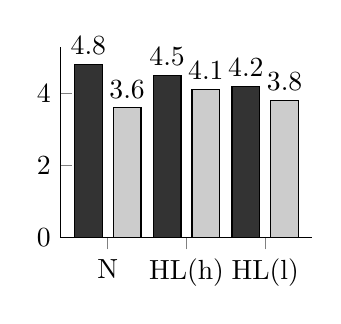
\begin{tikzpicture}
    \begin{axis}[ybar=4pt,
            x=1cm,
            ymin=0,
            symbolic x coords = {N,{HL(h)},{HL(l)}},
            xtick=data,
            axis lines*=left,
            nodes near coords,
            height=4cm,
            width=5cm,
            enlarge x limits=0.3
        ]
    \addplot[fill=black!80, draw=black] coordinates {
        (N,4.8)
        ({HL(h)},4.5)
        ({HL(l)},4.2)
    };
    
    \addplot[fill=black!20, draw=black] coordinates {
        (N,3.6)
        ({HL(h)},4.1)
        ({HL(l)},3.8)
    };
    \end{axis}
  \end{tikzpicture}
  \caption{All-new}
  \end{subfigure}%
  \begin{subfigure}[b]{.3\textwidth}
  \centering
  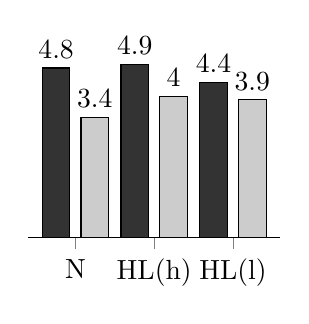
\begin{tikzpicture}
    \begin{axis}[ybar=4pt,
            x=1cm,
            ymin=0,
            symbolic x coords = {N,{HL(h)},{HL(l)}},
            xtick=data,
            axis x line*=bottom,
            axis y line=none,
            nodes near coords,
            height=4cm,
            width=5cm,
            enlarge x limits=0.3
        ]
    \addplot[fill=black!80, draw=black] coordinates {
        (N,4.8)
        ({HL(h)},4.9)
        ({HL(l)},4.4)
    };
    
    \addplot[fill=black!20, draw=black] coordinates {
        (N,3.4)
        ({HL(h)},4.0)
        ({HL(l)},3.9)
    };
    \end{axis}
  \end{tikzpicture}
  \caption{Object-given}
  \end{subfigure}%
  \begin{subfigure}[b]{.4\textwidth}
  \centering
  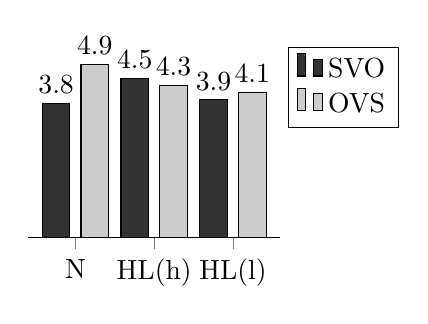
\begin{tikzpicture}
    \begin{axis}[ybar=4pt,
            x=1cm,
            ymin=0,
            symbolic x coords = {N,{HL(h)},{HL(l)}},
            xtick=data,
            axis x line*=bottom,
            axis y line=none,
            nodes near coords,
            height=4cm,
            width=5cm,
            enlarge x limits=0.3,
            legend pos=outer north east
        ]
    \addplot[fill=black!80, draw=black] coordinates {
        (N,3.8)
        ({HL(h)},4.5)
        ({HL(l)},3.9)
    };
    \addlegendentry{SVO}

    
    \addplot[fill=black!20, draw=black] coordinates {
        (N,4.9)
        ({HL(h)},4.3)
        ({HL(l)},4.1)
    };
    \addlegendentry{OVS}
    \end{axis}
  \end{tikzpicture}
  \caption{Object-given (pron.)}
  \end{subfigure}
%%please move the includegraphics inside the {figure} environment
%%\includegraphics[width=\textwidth]{figures/LalekoThecomplexityofwordorderchangeinaheritagelanguagesettingfinal-img002.svm}
 \end{figure}

In all-new contexts, Russian speakers in the control group displayed a significant preference towards SVO over SOV orders: $t (52.9) = 5.04$, $p < 0.01$. However, heritage speakers in both groups showed no such preference, accepting both SVO and SOV equally under broad focus (HL(h): $t (39.2) = 1.32$, $p > 0.05$; HL(l): $t (58) = 1.27$, $p > 0.05$). In object-given contexts with non-pronominal objects, the higher-proficiency heritage speakers and baseline controls displayed a preference for SVO over SOV orders: controls ($t (68.3) = 7.67$, $p < 0.01$), HL(h) ($t (40.6) = 4.16$, $p < 0.01$), while the lower-proficiency heritage speakers continued to treat SVO and SOV structures as interchangeable: $t (86.7) = 1.79$, $p > 0.05$. In pronominal constructions, however, the homeland speakers strongly preferred SOV orders to SVO orders ($t (62.9) = -5.86$, $p < 0.01$), while the heritage speakers found both options as equally acceptable, regardless of proficiency (HL(h): $t (59.06) = 0.72$, $p > 0.05$; HL(l): $t (86.97) = -0.75$, $p > 0.05$).

On across-group comparisons, SOV orders received significantly higher ratings in the higher-proficiency heritage language group compared to the baseline group both in all-new contexts ($t(48.1) = -1.6$, $p < 0.05$) and in object-given contexts ($t(73.8) = -2.04$, $p < 0.05$). Speakers in the lower-proficiency heritage speaker group converged with the controls in both conditions: all-new ($t(61.2) = -0.69$, 0 > 0.05), object-given ($t(87.8) = -1.73$, $p > 0.05$). Only in the pronominal condition, associated with an SOV preference over SVO in homeland speakers, did their ratings of SOV exceed those of the bilingual speakers: controls vs. HL(h) ($t(41.8) = 2.83$, $p < 0.01$), controls vs. HL(l) ($t(52.1) = 3.83$, $p < 0.01$).  

With respect to factors conditioning the SVO/SOV alternation in Russian, object givenness did not prove to be a crucial determinant in either homeland or heritage speakers at either level of proficiency: in all three groups, SOV orders were ranked uniformly in statistical terms regardless of their occurrence in all-new or object-given sentences: baseline ($t(68.9) = 0.58$, $p > 0.05$), HL(h) ($t(47.6) = 0.45$, $p > 0.05$), HL(l) ($t(67.2) = -0.3$, $p > 0.05$). However, ratings for SOV constructions were strongly affected by object type in homeland speakers, who significantly favored SOV orders with pronominal objects over non-pronominal objects: $t(62.9) = -8.2$, $p < 0.01$. Neither group of heritage speakers demonstrated significant effects with respect to object type (HL(h): $t(69.8) = -1.18$, $p > 0.05$; HL(l): $t(87.9) = -0.76$, $p > 0.05$).

\begin{figure}
\footnotesize
\begin{subfigure}[b]{.3\textwidth}
  \raggedright
  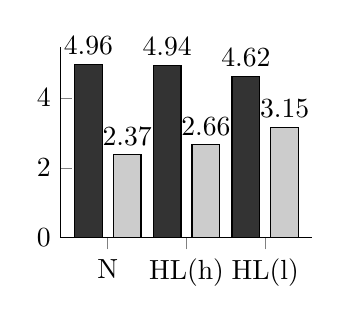
\begin{tikzpicture}
    \begin{axis}[ybar=4pt,
            x=1cm,
            ymin=0,
            symbolic x coords = {N,{HL(h)},{HL(l)}},
            xtick=data,
            axis lines*=left,
            nodes near coords,
            height=4cm,
            width=5cm,
            enlarge x limits=0.3
        ]
    \addplot[fill=black!80, draw=black] coordinates {
        (N,4.96)
        ({HL(h)},4.94)
        ({HL(l)},4.62)
    };
    
    \addplot[fill=black!20, draw=black] coordinates {
        (N,2.37)
        ({HL(h)},2.66)
        ({HL(l)},3.15)
    };
    \end{axis}
  \end{tikzpicture}
  \caption{All-new}
  \end{subfigure}%
  \begin{subfigure}[b]{.3\textwidth}
  \centering
  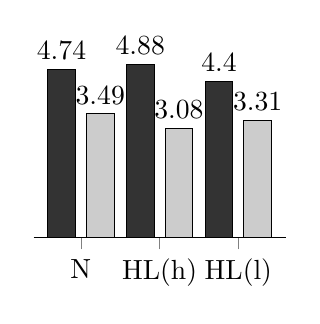
\begin{tikzpicture}
    \begin{axis}[ybar=4pt,
            x=1cm,
            ymin=0,
            symbolic x coords = {N,{HL(h)},{HL(l)}},
            xtick=data,
            axis x line*=bottom,
            axis y line=none,
            nodes near coords,
            height=4cm,
            width=5cm,
            enlarge x limits=0.3
        ]
    \addplot[fill=black!80, draw=black] coordinates {
        (N,4.74)
        ({HL(h)},4.88)
        ({HL(l)},4.4)
    };
    
    \addplot[fill=black!20, draw=black] coordinates {
        (N,3.49)
        ({HL(h)},3.08)
        ({HL(l)},3.31)
    };
    \end{axis}
  \end{tikzpicture}
  \caption{Object-given}
  \end{subfigure}%
  \begin{subfigure}[b]{.4\textwidth}
  \centering
  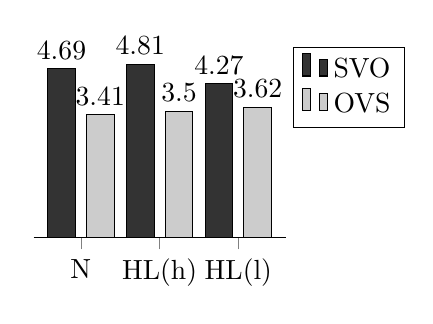
\begin{tikzpicture}
    \begin{axis}[ybar=4pt,
            x=1cm,
            ymin=0,
            symbolic x coords = {N,{HL(h)},{HL(l)}},
            xtick=data,
            axis x line*=bottom,
            axis y line=none,
            nodes near coords,
            height=4cm,
            width=5cm,
            enlarge x limits=0.3,
            legend pos=outer north east
        ]
    \addplot[fill=black!80, draw=black] coordinates {
        (N,4.69)
        ({HL(h)},4.81)
        ({HL(l)},4.27)
    };
    \addlegendentry{SVO}

    \addplot[fill=black!20, draw=black] coordinates {
        (N,3.41)
        ({HL(h)},3.5)
        ({HL(l)},3.62)
    };
    \addlegendentry{OVS}
    \end{axis}
  \end{tikzpicture}
  \caption{Object-given (pron.)}
  \end{subfigure}
\caption{\label{fig:laleko:3}Ratings for SVO and OSV sentences in all-new-information and object-given contexts}
\end{figure}

Finally, I turn to the analysis of OSV constructions. All groups showed a robust global preference towards SVO over OSV orders, both in all-new contexts (controls: $t(52.33) = 14.1$, $p < 0.01$; HL(h): $t(38.48) = 8.93$, $p < 0.01$; HL(l): $t(75.4) = 5.71$, $p < 0.01$) and in object-given nominal contexts (controls: $t(70.20) = 5.68$, $p < 0.01$); HL(h): $t(40.17) = 7.15$, $p < 0.01$; HL(l): $t(74.62) = 3.97$, $p < 0.01$). With pronominal objects, this tendency was observed in baseline and high-proficiency heritage speakers: controls ($t(84.02) = 5.33$, $p < 0.01$), HL(h) ($t(42.24) = 5.16$, $p < 0.01$). In lower-proficiency speakers, the difference between SVO and OSV orders with given pronominal objects did not reach significance at the same threshold, but was still significant at a weaker level: $t(83.14) = -1.51$, $p < 0.05$.

Despite exhibiting a preference for the canonical SVO pattern over OSV in all conditions, the homeland speakers were highly sensitive to object givenness in their ratings of OSV orders and gave significantly higher ratings to OSV in object-given contexts compared to all-new contexts: $t(98.77) = -4.07$, $p < 0.01$. In contrast, the heritage speakers were not sensitive to object givenness in their ratings of OSV orders at either proficiency level: HL(h) ($t(69.96) = -1.19$, $p > 0.05$), HL(l) ($t(87.57) = -0.49$, $p > 0.05$). Furthermore, object type (i.e., pronominal or not) did not matter for any of the three groups: homeland ($t(99.99) = 0.27$, $p > 0.05$), HL(h) ($t(69.99) = -1.21$, $p > 0.05$), HL(l) ($t(87.14) = -0.99$, $p > 0.05$). In what follows, I discuss these results and their implications.

\section{Discussion and conclusions}\label{sec:laleko:5}

The study examined the dynamics of word order change in heritage Russian, with the larger aim of assessing to what extent the trajectory of change in this domain conforms to the broad conception of heritage language change as successive simplification of structures and structure-building processes along the proficiency scale, emerging from a rich body of previous work on morphosyntactic restructuring in heritage languages. Experimental data from heritage Russian speakers at two levels of proficiency and a group of homeland speakers were analyzed to identify principles utilized in the respective linguistic varieties for the syntactic encoding of information-structural categories: focus, involved in the alternation between SVO and OVS orders, and givenness, implicated in the variation among SVO, SOV, and OSV orders. Starting with the theoretically established premise that Russian builds on an SVO tree to derive OVS, SOV, and OSV structures, and that these structures occur in particular, predetermined discourse contexts, the main goal of the study was to gauge the stability of the derived orders across two levels of heritage language proficiency and to trace changes in principles guiding their occurrence.

Broadly, the results do not support the conceptualization of heritage language change as a process of inexorable simplification. Instead, the findings point to a more nuanced picture of word order change, whereby patterns of simplification in some domains of the word order system intersect with trends towards preservation and even increase of complexity in its other areas. In the discussion of the results that follows, I will first outline and comment on the manifestations of reductive change, and then take stock of areas of stability and amplified variability in the heritage language word order system.

With respect to the OVS constructions, employed for the encoding of subject focus in Russian, the trajectory of change emerging from the ratings of homeland speakers and heritage speakers at two discrete points on the proficiency spectrum renders support to a model of heritage language change as a linearly progressing process of reduction in syntactic variability. While heritage speakers at the higher end of the proficiency spectrum display the same grammaticality effects as homeland speakers, these effects dissipate with decreasing proficiency. Furthermore, heritage speakers in both groups display a diminished acceptance of OVS, preferring instead the canonical SVO structures in the same contexts. These patterns are indicative of a weakening of OVS in the heritage language and its replacement with the canonical SVO pattern in contexts in which both structures co-exist in the baseline system. In effect, this change may be viewed as a \textit{narrowing} of a set of linguistic options available for the marking of a particular distinction in favor of the least restrictive, minimally specified variant that constitutes a shared default between the bilinguals’ two word order systems.

Data on the distribution of OSV orders in Russian present a less clear case of simplification-driven change in the heritage language word order system. Since no quantitative reduction in the acceptability of these orders was observed – either in the group of heritage speakers compared to homeland speakers, or as a function of heritage language proficiency – it would be premature to conclude that these non-canonical structures are on a path to elimination from the heritage Russian word order system. While showing no immediate signs of quantitative decrease, the results are nevertheless indicative of a change affecting the contextual principles on the occurrence of OSV orders in the heritage language: the robust effects of object givenness attested in the homeland variety are absent in the heritage speakers’ ratings regardless of proficiency. In this sense, the findings partially mirror the pattern of change observed for OVS structures, with an important difference concerning the proficiency level at which the loss of the relevant information-structural effect is observed. Recall that the deactivation of focus as a conditioning factor for OVS structures was attested only in the lower-proficiency heritage group, with advanced speakers performing on par with homeland speakers on this dimension. In contrast, the unlinking of OSV from object givenness is discernible at both proficiency levels. This contrast highlights a previously observed asymmetry between the effects of two distinct facets of information structure on word order, whereby the more informationally and prosodically salient categories like focus and contrast seem more resilient to change than categories associated with topicality and anaphoricity (see \citealt{Laleko2021}: 719--721 for discussion). If on the right track, these results advocate for a more fine-grained approach to the study of the syntax-discourse interface phenomena than one commonly used in empirical research, where “information structure” often stands as a blanket term rather than a composite, multi-layered category comprised of an array of phenomena with distinct effects on linguistic structure and interpretation.

Finally, the patterns of homeland and heritage speakers’ ratings obtained for SOV constructions provide the strongest evidence against an overly broad conceptualization of heritage language word order change as a unidirectional process of convergence towards the SVO template. Even at the lower proficiency level, heritage speakers showed no decrease in acceptability for SOV orders with nominal objects, fully converging with homeland speakers on SOV constructions in both all-new and object-given contexts – a pattern indicative of their high stability in bilingual grammars. Moreover, the fact that the higher-proficiency heritage speakers displayed more favorable judgments of SOV orders than homeland speakers in the same contexts speaks not only to stability, but also to an enhancement and strengthening of this pattern in these more established heritage grammars. The fact that the higher-proficiency speakers in this study rated SOV structures on par with SVO structures in all-new contexts is particularly notable in this regard: in effect, this development constitutes an expansion in the set of defaults in the heritage language word order system, compared to the baseline system. This pattern of change stands in sharp contrast with the view of heritage language change as a process of contraction to a single default (e.g., of the type observed in this study for SVO/OVS alternation), suggesting that multiple defaults are, in principle, permitted in restructured grammars and prompting further research into factors responsible for their emergence. In the remainder of this concluding section, I frame the discussion around two particular implications of these results, concentrating primarily on avenues in which they may inform future research on heritage language change.

Viewed in the context of the bulk of existing studies, the observed “elevation” of the SOV pattern to the status of unmarked, discourse-neutral order in the grammars of English-dominant Russian speakers constitutes a rarely documented case of non-transfer-induced complexity-preserving change. While several prior heritage language studies have reported evidence of complexification in various domains of heritage language structure, manifested as a strengthening of a particular non-canonical order or construction in a heritage language variety otherwise undergoing reductive change (e.g., \citealt{AalberseMoro2014, AalberseZhouAndringa2017, BrehmerUsanova2015, vanOschSleeman2018Subject}), virtually all of such hitherto reported developments have been attributed to cross-linguistic influence from the societally dominant language. In this light, the observed retention and strengthening of SOV, a structure that is impossible in English, in heritage Russian provides a strong impetus for continued research on sources of complexity-preserving change operating in contact situations but falling outside of clear transfer effects. The present results bring two such factors into the spotlight – one having to do with the internal composition of the Russian word order system, and the other stemming more globally from the cognitive and communicative principles that govern constituent placement in natural languages. Focusing narrowly on the internal dynamic of the Russian language, the marked contrast between the frequencies of VO and OV orders observed for its written/formal and spoken/colloquial registers, with preverbal objects ranging between 7--9\% in scientific speech and up to 60\% in colloquial speech, has prompted some scholars to characterize spoken Russian as undergoing a typological shift from SVO to SOV (\citealt{Slioussar2007}). Under this view, the expansion of the SOV pattern in heritage Russian may be seen as an instance of input-driven change that builds on and amplifies incipient changes already happening in the baseline (\citealt{Polinsky2018}); the fact that this development in the heritage language occurs despite the potentially constraining effects of ambient language transfer and seems resistant to them attests to its potency as a mechanism of change.\footnote{It should be noted that input-related properties may also be implicated in the observed quantitative reduction of OVS structures to mark subject focus in heritage Russian. It has been observed that colloquial Russian differs from standard Russian in the syntactic encoding of new information focus: while usually expressed clause-finally in written language, focus is often preposed in spoken registers (\citealt{KrylovaKhavronina1986, Yokoyama1986}).} From a more general typological perspective, the pattern of SOV strengthening in spoken Russian, including Russian as a heritage language, may be a reflection of the basic evolutionary and cognitive principles that account for the overall preference for SOV ordering in human language (\citealt{Dryer2013Order, Newmeyer2000}) and have been claimed to be engaged productively in the formation of emerging linguistic systems and in spontaneous communication, including under conditions of limited input (\citealt{Goldin-Meadow2003, NapoliSutton-Spence2014}). If on the right track, these proposals warrant a closer look at the fate of SOV structures in heritage languages – systems modeled on reduced and variably accessible input. Such investigations would be particularly welcome for languages with an otherwise restricted occurrence of SOV, e.g. heritage English, as a way of teasing apart the issue of universal constituent placement principles from language-internal, diachronically changing pressures – a task that cannot be accomplished in this study.

A second, related implication emerging from the patterns of results obtained for SOV structures concerns the construct of heritage language proficiency and its conceptualization and operationalization in heritage language research. Since the inception of the field, the study of heritage language properties has focused heavily on morphosyntax, and models of language proficiency proposed to account for the systematic variability in the linguistic abilities in heritage speakers, most typically scaled from low to high proficiency based on a degree of distance from the baseline system, have been calibrated first and foremost to aspects of grammatical variation, with a tacit assumption that other domains of language would follow suit. The results presented here do not support this assumption, suggesting instead that the extent of convergence between the heritage and homeland varieties may vary, and sometimes principally, for individual linguistic domains. In this study, which relied on morphosyntactic variables for proficiency assessment, heritage systems with deeper grammatical restructuring were more baseline-like in their word order properties than those with more stable grammars. While counter-intuitive under traditional conceptions of heritage language proficiency, such diverging trajectories of change across different linguistic sub-domains – morphosyntax and word order in particular – have been documented in other studies of language shift. For instance, a similar pattern of proficiency split was attested in shifting speakers of Even, a fixed head-final SOV language spoken in northeastern Russia. The less proficient speakers resisted word order change while omitting inflectional morphology; in contrast, the higher-proficiency speakers exhibited word order changes while maintaining the grammar of case \citep{KantarovichNesterova2021}. Taken together with other studies that document innovations in stable and successfully maintained heritage languages (\citealt{AalberseMoro2014, AalberseZhouAndringa2017}), the results obtained here raise the question of whether morphosyntactic stability may serve as a precursor of change in language domains that are especially responsive to communicative pressures. One prediction of this hypothesis would be that the more established heritage grammars, as measured by grammatical accuracy, may be associated with greater heritage language use and exposure, leading in turn to a higher degree of innovations arising as a result of the language developing in a new environment and under different communicative conditions.

If on the right track, this observation encourages a closer look at proficiency-based variation in heritage languages as an opportunity to expand our conceptualization of heritage language change in order to arrive at a more fine-grained differentiation among distinct mechanisms contributing to its genesis, teasing apart elements of change arising due to quantitative reduction in the linguistic input from those stemming from propagation of features and norms entrenched in qualitatively different, yet abundantly present, input. With respect to the data discussed here, it appears that while elements of simplification are certainly a part of the process of change, they are not, at least in this case, the only relevant dynamic of change in the heritage language varieties under examination.

\printbibliography[heading=subbibliography,notkeyword=this]
\end{document} 
